\documentclass[12pt]{article}

%% ---------------------------------------------------------------------------
%% 10-703 Homework 3 submission template
%% Students: only type at the "% YOUR SOLUTION HERE" markers inside each box.
%% ---------------------------------------------------------------------------

\usepackage[margin=1in]{geometry}
\usepackage{amsmath, amssymb}
\usepackage{graphicx}
\usepackage{array}
\usepackage{xcolor}
\usepackage[most]{tcolorbox}
\usepackage{lastpage}
\usepackage[colorlinks=true, linkcolor=red, urlcolor=blue]{hyperref}

\setlength{\parindent}{0pt}
\setlength{\parskip}{6pt}

%% ---------------------------------------------------------------------------
%% Staff: point values. The handout only fixes the per-problem totals, so the
%% per-box values are left empty. Fill one in (e.g. \newcommand{\ptsClip}{8})
%% and " (8 pts)" is appended to that heading automatically.
%% ---------------------------------------------------------------------------
\newcommand{\ptsPPO}{50}
\newcommand{\ptsTDthree}{35}
\newcommand{\ptsSAC}{15}

\newcommand{\ptsClip}{}        % 1.4.1
\newcommand{\ptsKL}{}          % 1.4.2
\newcommand{\ptsHighClip}{}    % 1.5.1
\newcommand{\ptsLowClip}{}     % 1.5.3
\newcommand{\ptsFullOff}{}     % 1.6.1
\newcommand{\ptsHalfOff}{}     % 1.6.2
\newcommand{\ptsTDEval}{}      % 2.5 (evaluation)
\newcommand{\ptsTDSmooth}{}    % 2.5 (target policy smoothing)
\newcommand{\ptsTDDelay}{}     % 2.6
\newcommand{\ptsSACEval}{}     % 3.3
\newcommand{\ptsSACUTD}{}      % 3.4
\newcommand{\ptsSACBackup}{}   % 3.5

\makeatletter
\newcommand{\showpts}[1]{%
  \begingroup\edef\@tmp{#1}\ifx\@tmp\@empty\else\ (#1 pts)\fi\endgroup}
\makeatother

%% ---------------------------------------------------------------------------
%% Headings and answer boxes
%% ---------------------------------------------------------------------------
\newcommand{\problem}[2]{\section*{#1\showpts{#2}}}
\newcommand{\subproblem}[2]{\subsection*{#1\showpts{#2}}}
\newcommand{\boxlabel}[1]{\par\textbf{#1}\par\nopagebreak}

% Fixed-height answer box. Argument = height. Do not change the heights.
\newtcolorbox{answerbox}[1]{%
  colback=white, colframe=black, height=#1, valign=top,
  before skip=4pt, after skip=8pt}

% Small inline box (collaborators, fill in the blank).
\newcommand{\inlinebox}[2]{%
  \tcbox[colback=white, colframe=black, sharp corners, boxrule=0.4mm,
         nobeforeafter, box align=center, width=#1, height=0.75cm,
         left=2pt, right=2pt, top=1pt, bottom=1pt, tcbox width=forced center]{#2}}

\begin{document}

%% ===========================================================================
%% Instructions
%% ===========================================================================
\begin{center}
  {\huge\textsc{Homework 3 Template}}
\end{center}
\vspace{6pt}

Use this template to record your answers for Homework 3. Add your answers using \LaTeX{} and
then save your document as a PDF to upload to Gradescope. You are required to use this
template to submit your answers. \textbf{You should not alter this template in any way} other
than to insert your solutions. You must submit all \pageref{LastPage} pages of this template to Gradescope.
Do not remove the instructions page(s). Altering this template or including your solutions
outside of the provided boxes can result in your assignment being graded incorrectly. You
may lose points if you do not follow these instructions.

Instructions to upload code have been provided in the handout.

\section*{Instructions for Specific Problem Types}

On this homework, you must fill in the box for each problem; please make sure your final
answer is fully included in the given space. \textbf{Do not change the size of the box provided.}
For plot boxes, insert the figures generated by \texttt{runner.py} and scale them so that they
fit entirely inside the box. For short answer questions you should \textbf{not} include your
work in your solution. Only provide an explanation if specifically asked. Otherwise, your
assignment may not be graded correctly, and points may be deducted from your assignment.

\hspace{1.5em}\textbf{Fill in the blank:} What is the course number?

\hspace{1.5em}\inlinebox{3cm}{%
10-703
}

\clearpage
%% ===========================================================================
%% Problem 0
%% ===========================================================================
\section*{Problem 0: Collaborators}

Enter your team's names and Andrew IDs in the boxes below. If you do not do this, you
may lose points on your assignment.

\vspace{6pt}
\renewcommand{\arraystretch}{1.9}
\begin{tabular}{@{}l@{\ }l@{\quad}l@{\ }l@{}}
Name 1: & \inlinebox{3.6cm}{%
Arnav Goyal
} & Andrew ID 1: & \inlinebox{3.6cm}{%
arnavgoy
} \\
Name 2: & \inlinebox{3.6cm}{%
Kushal Kejriwal
} & Andrew ID 2: & \inlinebox{3.6cm}{%
kkejriwa
} \\
Name 3: & \inlinebox{3.6cm}{%
Vineeth Bhat
} & Andrew ID 3: & \inlinebox{3.6cm}{%
vineethb
} \\
\end{tabular}
\renewcommand{\arraystretch}{1}

\clearpage
%% ===========================================================================
%% Problem 1: PPO
%% ===========================================================================
\problem{Problem 1: Proximal Policy Optimization}{\ptsPPO}

Problems 1.1--1.3 are graded from your code submission (\texttt{ppo\_agent.py}) and have no
written component.

\subproblem{1.4.1 Clipped Objective}{\ptsClip}
\boxlabel{Plots}
\begin{answerbox}{10cm}
% TODO: Put your figures, e.g.
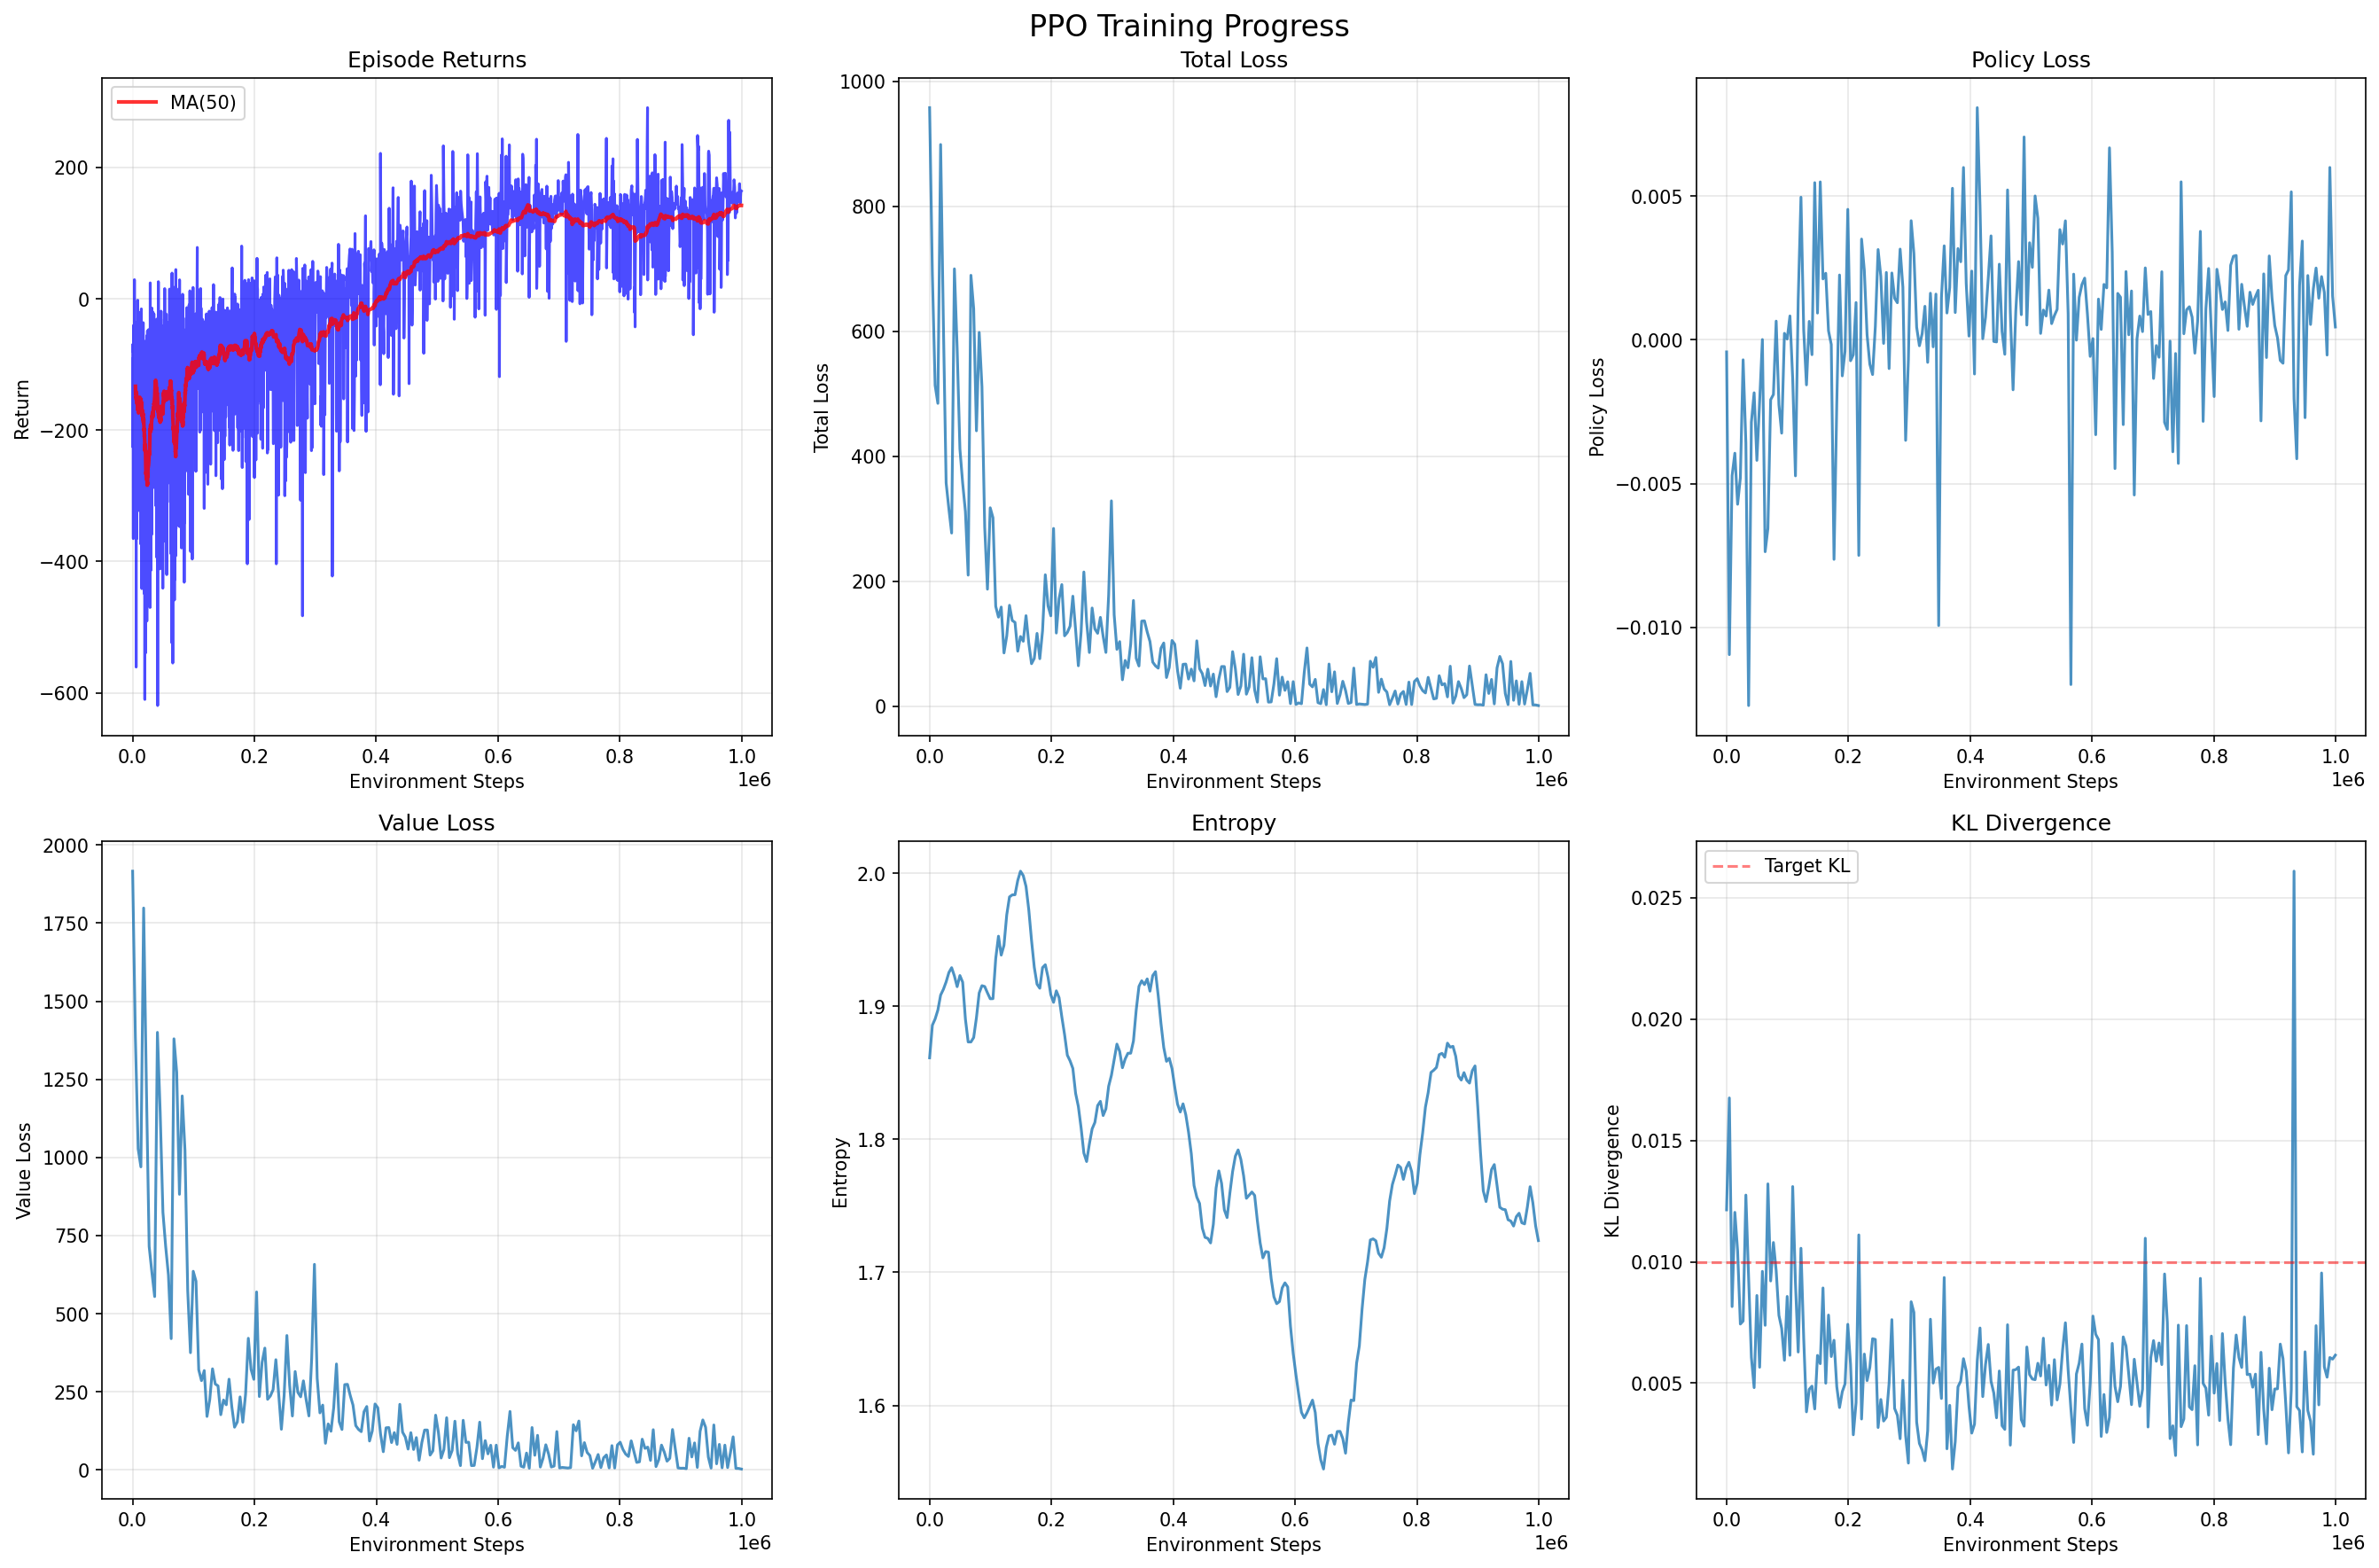
\includegraphics[width=\linewidth,height=8.5cm,keepaspectratio]{src/runs/ppo_images/1.4.1_training_curves.png}
% YOUR SOLUTION HERE
\end{answerbox}
\boxlabel{Final performance}
\begin{answerbox}{2.5cm}
\emph{Training:} Ending MA(50) = $142.3$. Training returns (max/mean/min): all episodes $291.1/-56.5/-619.4$; last 50 $271.9/142.3/-20.4$ (SD $51.5$). \textbf{Note}: $\text{Max} > 200$.\par
\emph{Evaluation:} Best checkpoint, deterministic actions: $214.9\pm 65.4$ (mean $\pm$ SD).\par
\end{answerbox}

\clearpage
\subproblem{1.4.2 KL-Penalized Objective}{\ptsKL}
\boxlabel{Plots}
\begin{answerbox}{9cm}
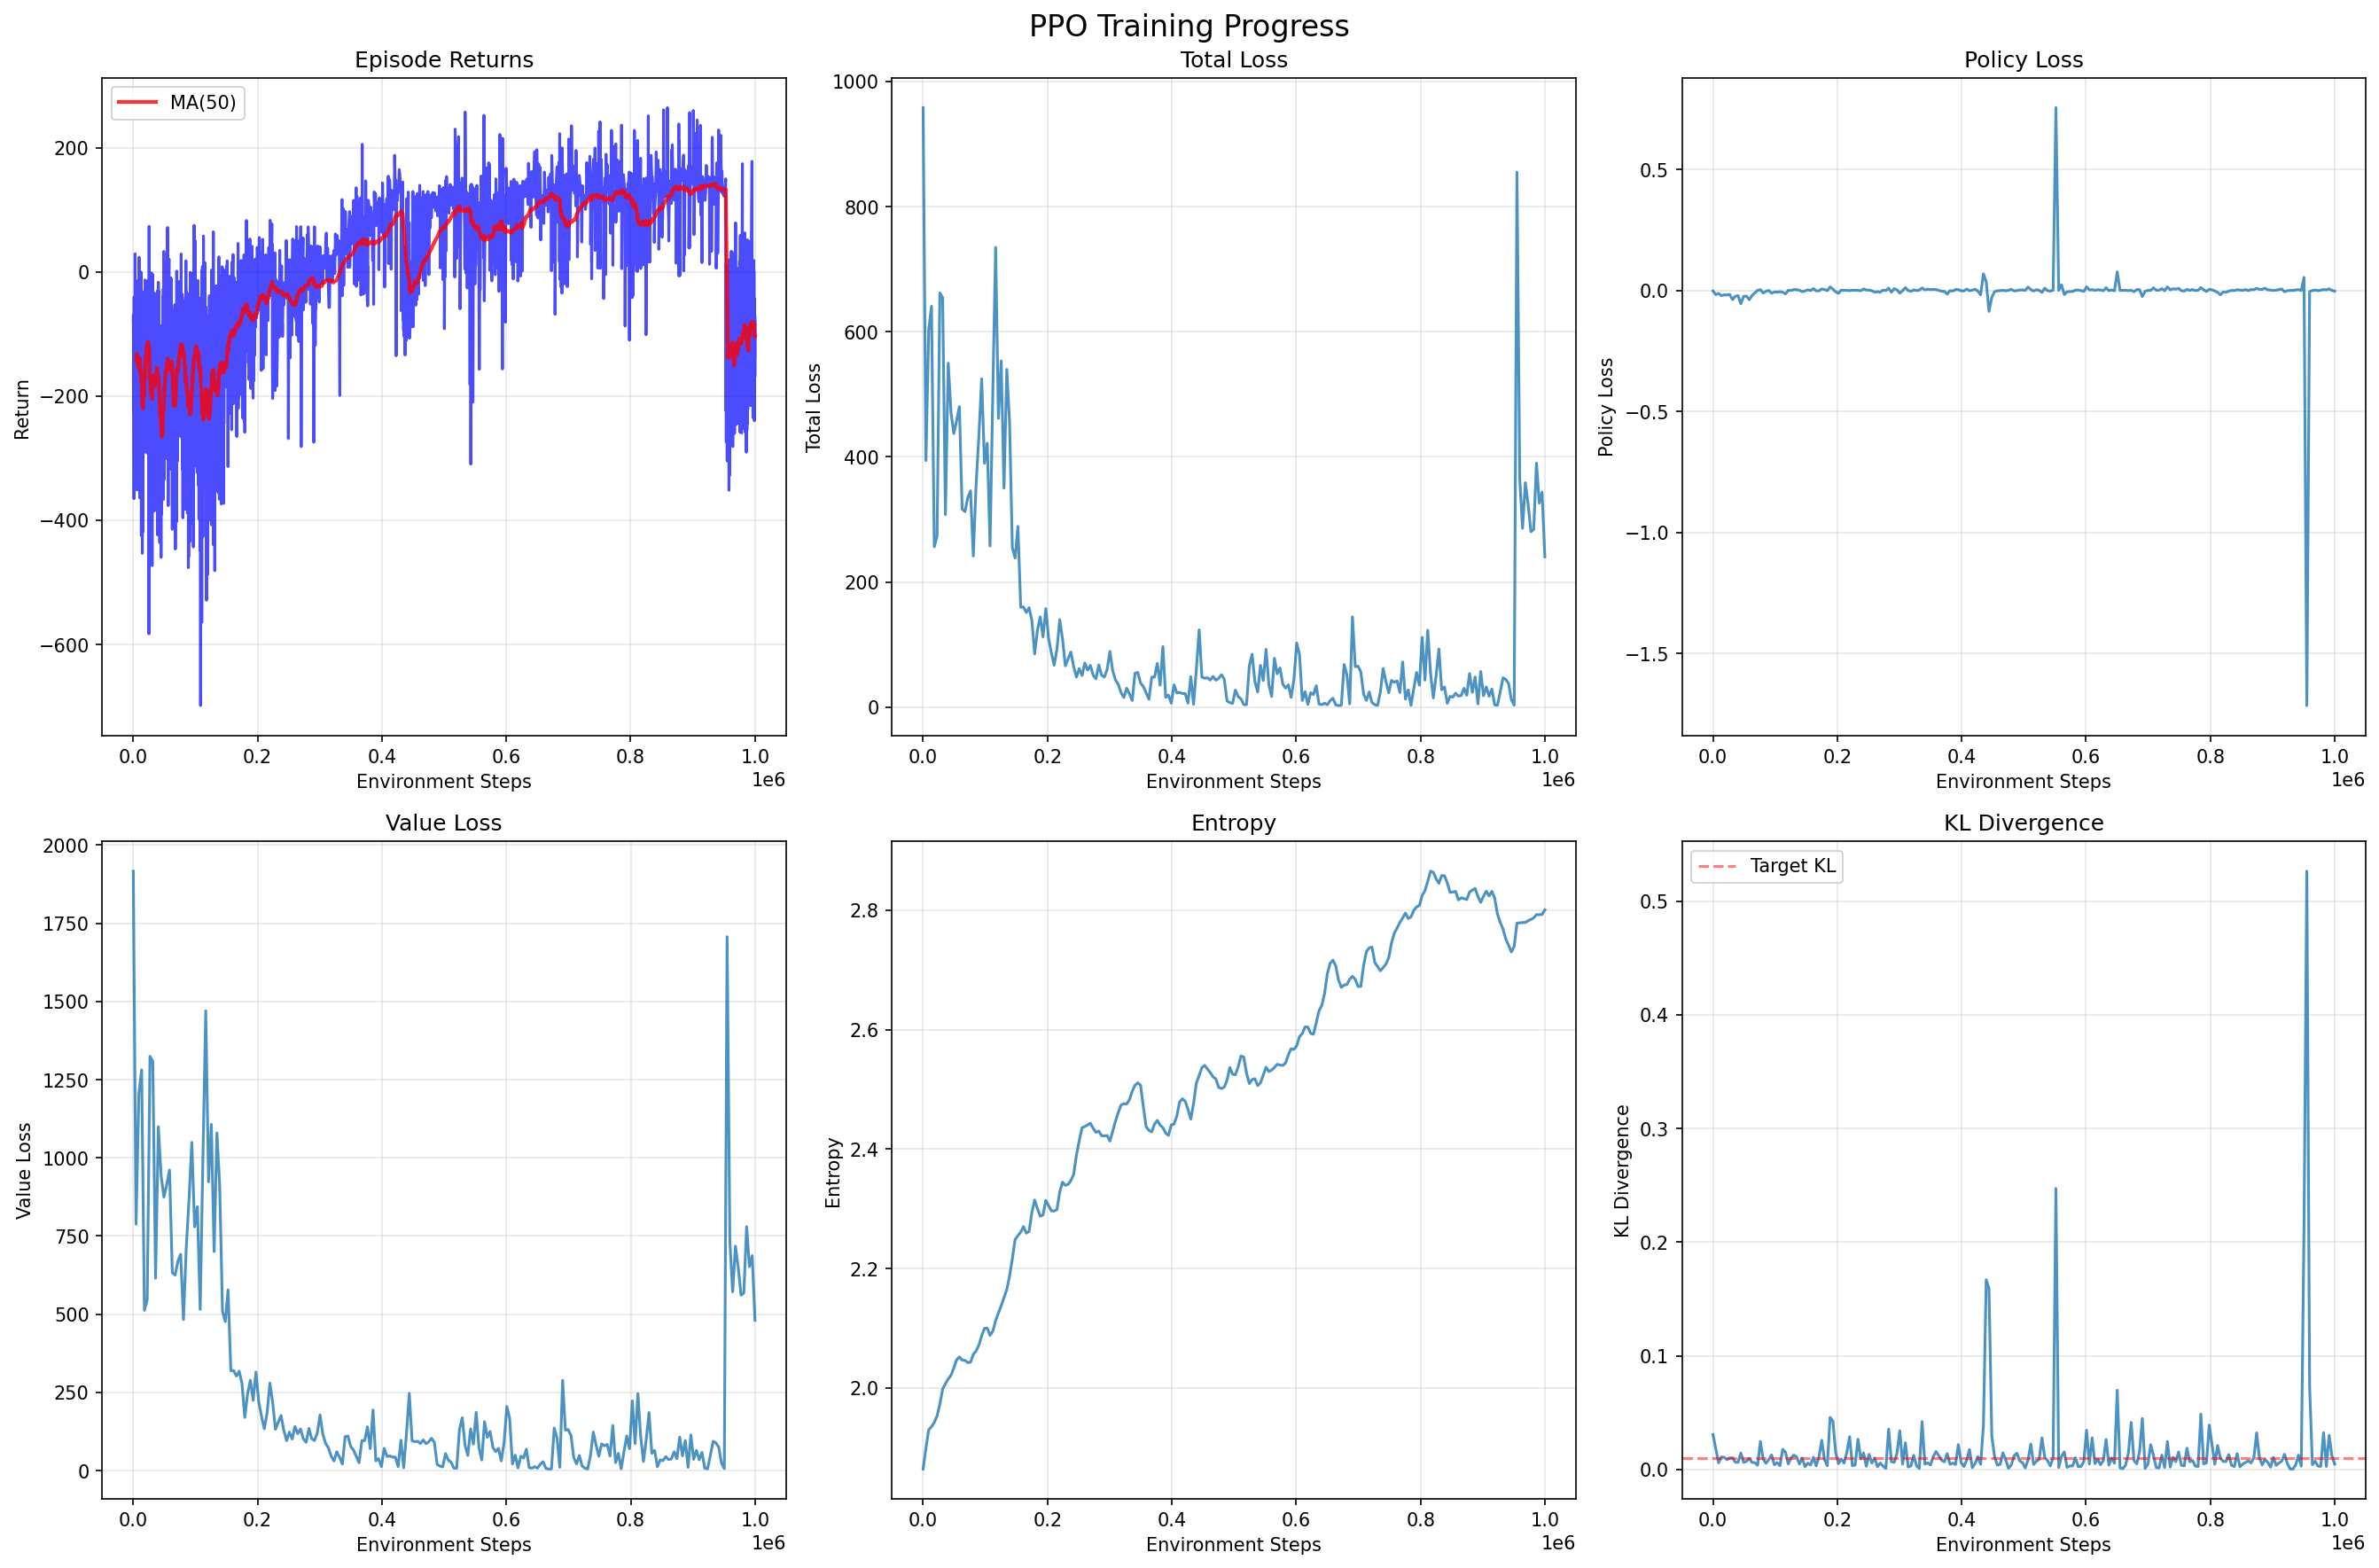
\includegraphics[width=\linewidth,height=8.5cm,keepaspectratio]{src/runs/ppo_images/1.4.2_training_curves.png}
\end{answerbox}
\boxlabel{Final performance}
\begin{answerbox}{2cm}
\emph{Training:} Ending MA(50) = $-104.5$. Training returns (max/mean/min): all episodes $264.5/-74.5/-698.4$; last 50 $18.6/-104.5/-239.7$ (SD $54.2$).\par
\emph{Evaluation:} Best checkpoint, deterministic actions: $240.1\pm 70.9$ (mean $\pm$ SD).\par
\end{answerbox}
\boxlabel{Reflection: clipping vs.\ KL penalty}
\begin{answerbox}{6.5cm}
Clipping in our trial was more stable in terms of avoiding large KL divergences and large loss spikes. The KL run had a late KL spike above $0.5$, as well as sharp increases in policy and value losses while clipping remained relatively stabler.  Clipping was also more stable in the sense that it reached a higher MA(50) of $142.3$ while KL later collapsed to $-104.5$. \emph{However,} KL's best checkpoint evaluated better at $240.1$ compared to clipping's $214.9$.

Clipping's adv. are simplicity and fewer large KL and loss spikes and better retention of training performance, while its disadv. is that it only removes incentives for excessive probability changes and does not directly constrain overall policy divergence. The KL penalty explicitly discourages divergence and produced a better best checkpoint in our run, but requires adapting $\beta$. If the penalty is too weak, disruptive updates can occur and if its too strong, learning can slow. \emph{Neither approach guarantees small updates}.
\end{answerbox}

\clearpage
\subproblem{1.5.1 High Clipping Threshold ($\epsilon = 0.3$)}{\ptsHighClip}
\boxlabel{Plots}
\begin{answerbox}{9cm}
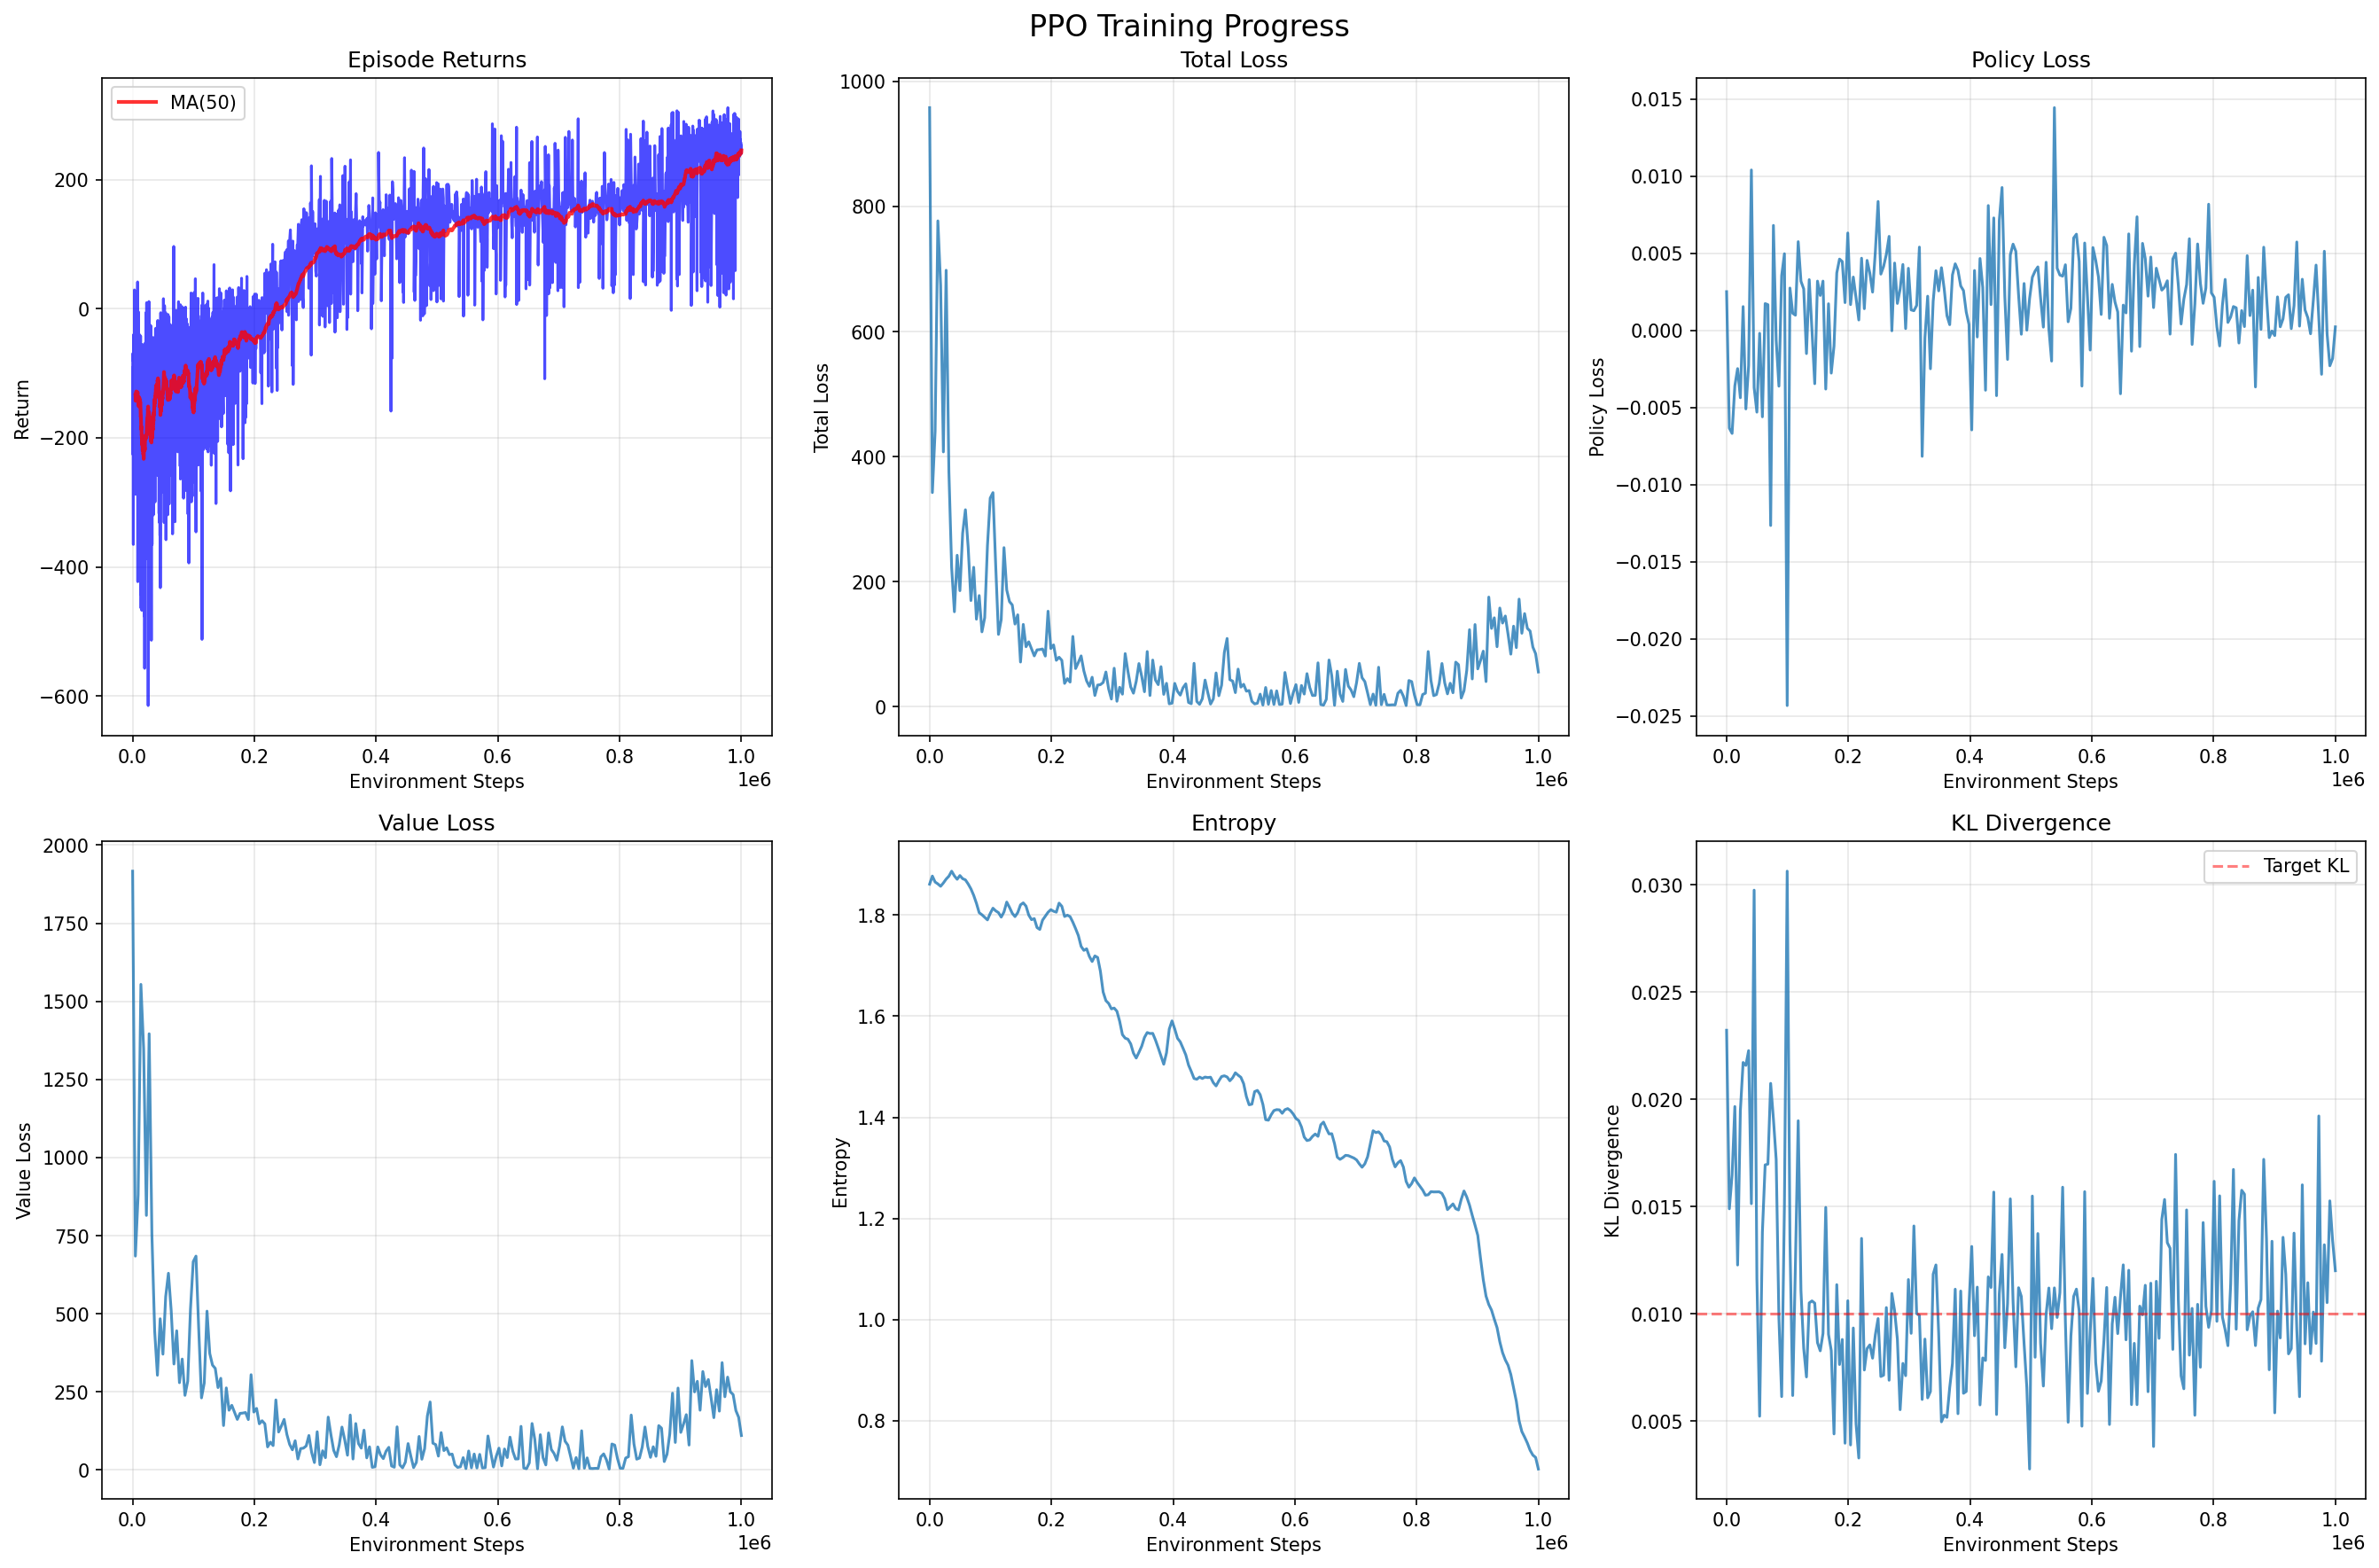
\includegraphics[width=\linewidth,height=8.5cm,keepaspectratio]{src/runs/ppo_images/1.5.1_training_curves.png}
\end{answerbox}
\boxlabel{Final returns}
\begin{answerbox}{2cm}
\emph{Training:} Ending MA(50) = $245.3$. Training returns (max/mean/min): all episodes $311.5/2.8/-614.8$; last 50 $302.6/245.3/15.3$ (SD $53.9$).\par
\emph{Evaluation:} Best checkpoint, deterministic actions: $254.2\pm 57.0$ (mean $\pm$ SD).\par
\end{answerbox}
\boxlabel{Discussion}
\begin{answerbox}{6.5cm}
With $\epsilon=0.3$, learning was faster than 1.4.1 and the ending MA(50) increased from $142.3$ to $245.3$, and best-checkpoint evaluation increased from $214.9$ to $254.2$. KL was generally around $0.01$, compared with roughly $0.005$ for the 1.4.1, so there were larger policy changes. Lastly, last-50 return SD was similar ($53.9$ versus $51.5$).

For positive advantages, clipping removes the incentive to increase $r_t$ beyond $1+\epsilon$ and for negative advantages, it removes the incentive to decrease $r_t$ below $1-\epsilon$. Larger $\epsilon$ therefore allows stronger changes before clipping comes in, making the realized objective closer to the unclipped policy gradients. 

The trade-off is faster learning versus potentially less stable updates in terms of loss spikes and KL divergences. In our case, the run benefited from the larger threshold while remaining relatively stable.
\end{answerbox}

\clearpage
\subproblem{1.5.3 Low Clipping Threshold ($\epsilon = 0.05$)}{\ptsLowClip}
\boxlabel{Plots}
\begin{answerbox}{9cm}
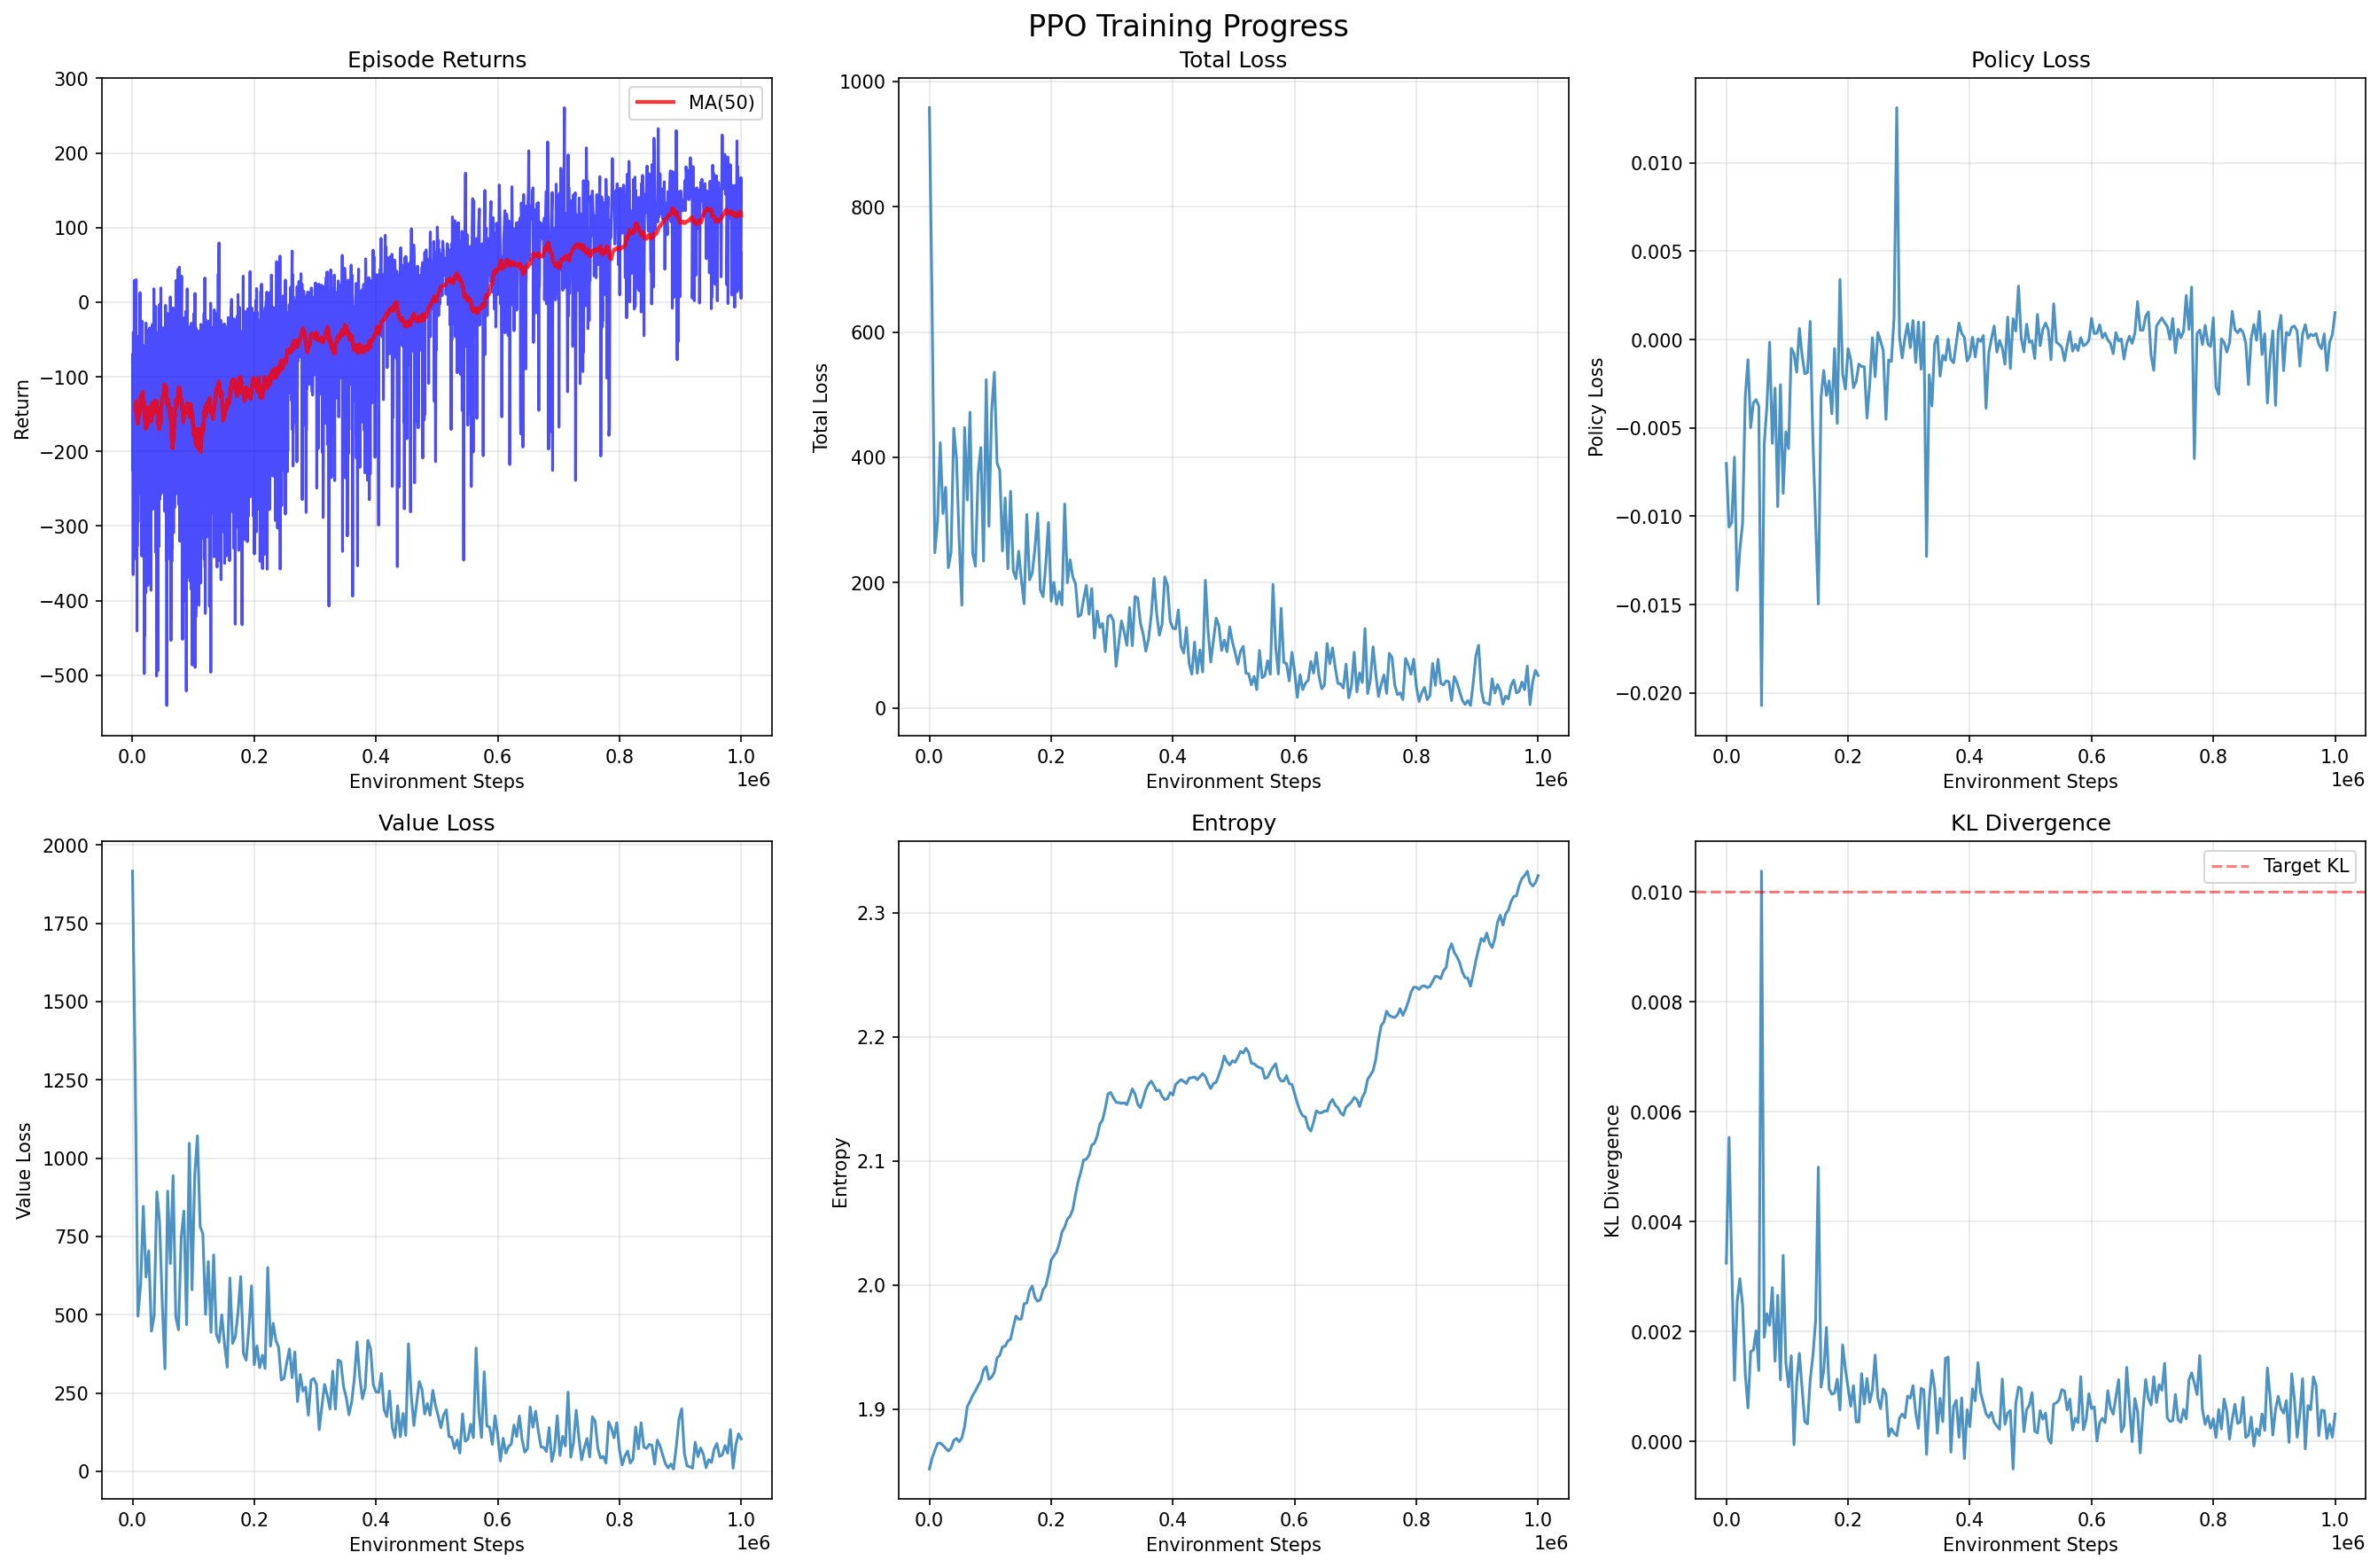
\includegraphics[width=\linewidth,height=8.5cm,keepaspectratio]{src/runs/ppo_images/1.5.2_training_curves.png}
\end{answerbox}
\boxlabel{Final returns}
\begin{answerbox}{2cm}
\emph{Training:} Ending MA(50) = $115.9$. Training returns (max/mean/min): all episodes $260.8/-73.0/-540.8$; last 50 $224.2/115.9/-6.8$ (SD $63.4$).\par
\emph{Evaluation:} Best checkpoint, deterministic actions: $137.4\pm 115.9$ (mean $\pm$ SD).\par
\end{answerbox}
\boxlabel{Discussion}
\begin{answerbox}{6.5cm}
With $\epsilon=0.05$, learning was slower and the ending MA(50) fell to $115.9$ and best-checkpoint evaluation to $137.4$, as compared to the $142.3$ and $214.9$ (resp.) for 1.4.1. After early training, KL was mostly below $0.002$, and the policy objective fluctuated less. This indicates more stable policy updates, but does not directly indicate consistent returns since the last-50 return SD increased from $51.5$ (1.4.1) to $63.4$.

The narrower clipping interval removes incentives for further useful probability changes sooner therefore limiting / slowing down progress. So, smaller updates can improve policy update stability while reducing learning speed and final performance (i.e., with a fixed compute budget). 

In higher-dimensional or more complex environments, conservative updates may help avoid disruption owing to higehr plausibilit for instability. However, excessively tight clipping can still prevent sufficient learning within the available compute budget.
\end{answerbox}

\clearpage
\subproblem{1.6.1 Full Off-Policy PPO}{\ptsFullOff}
\boxlabel{Plots}
\begin{answerbox}{9cm}
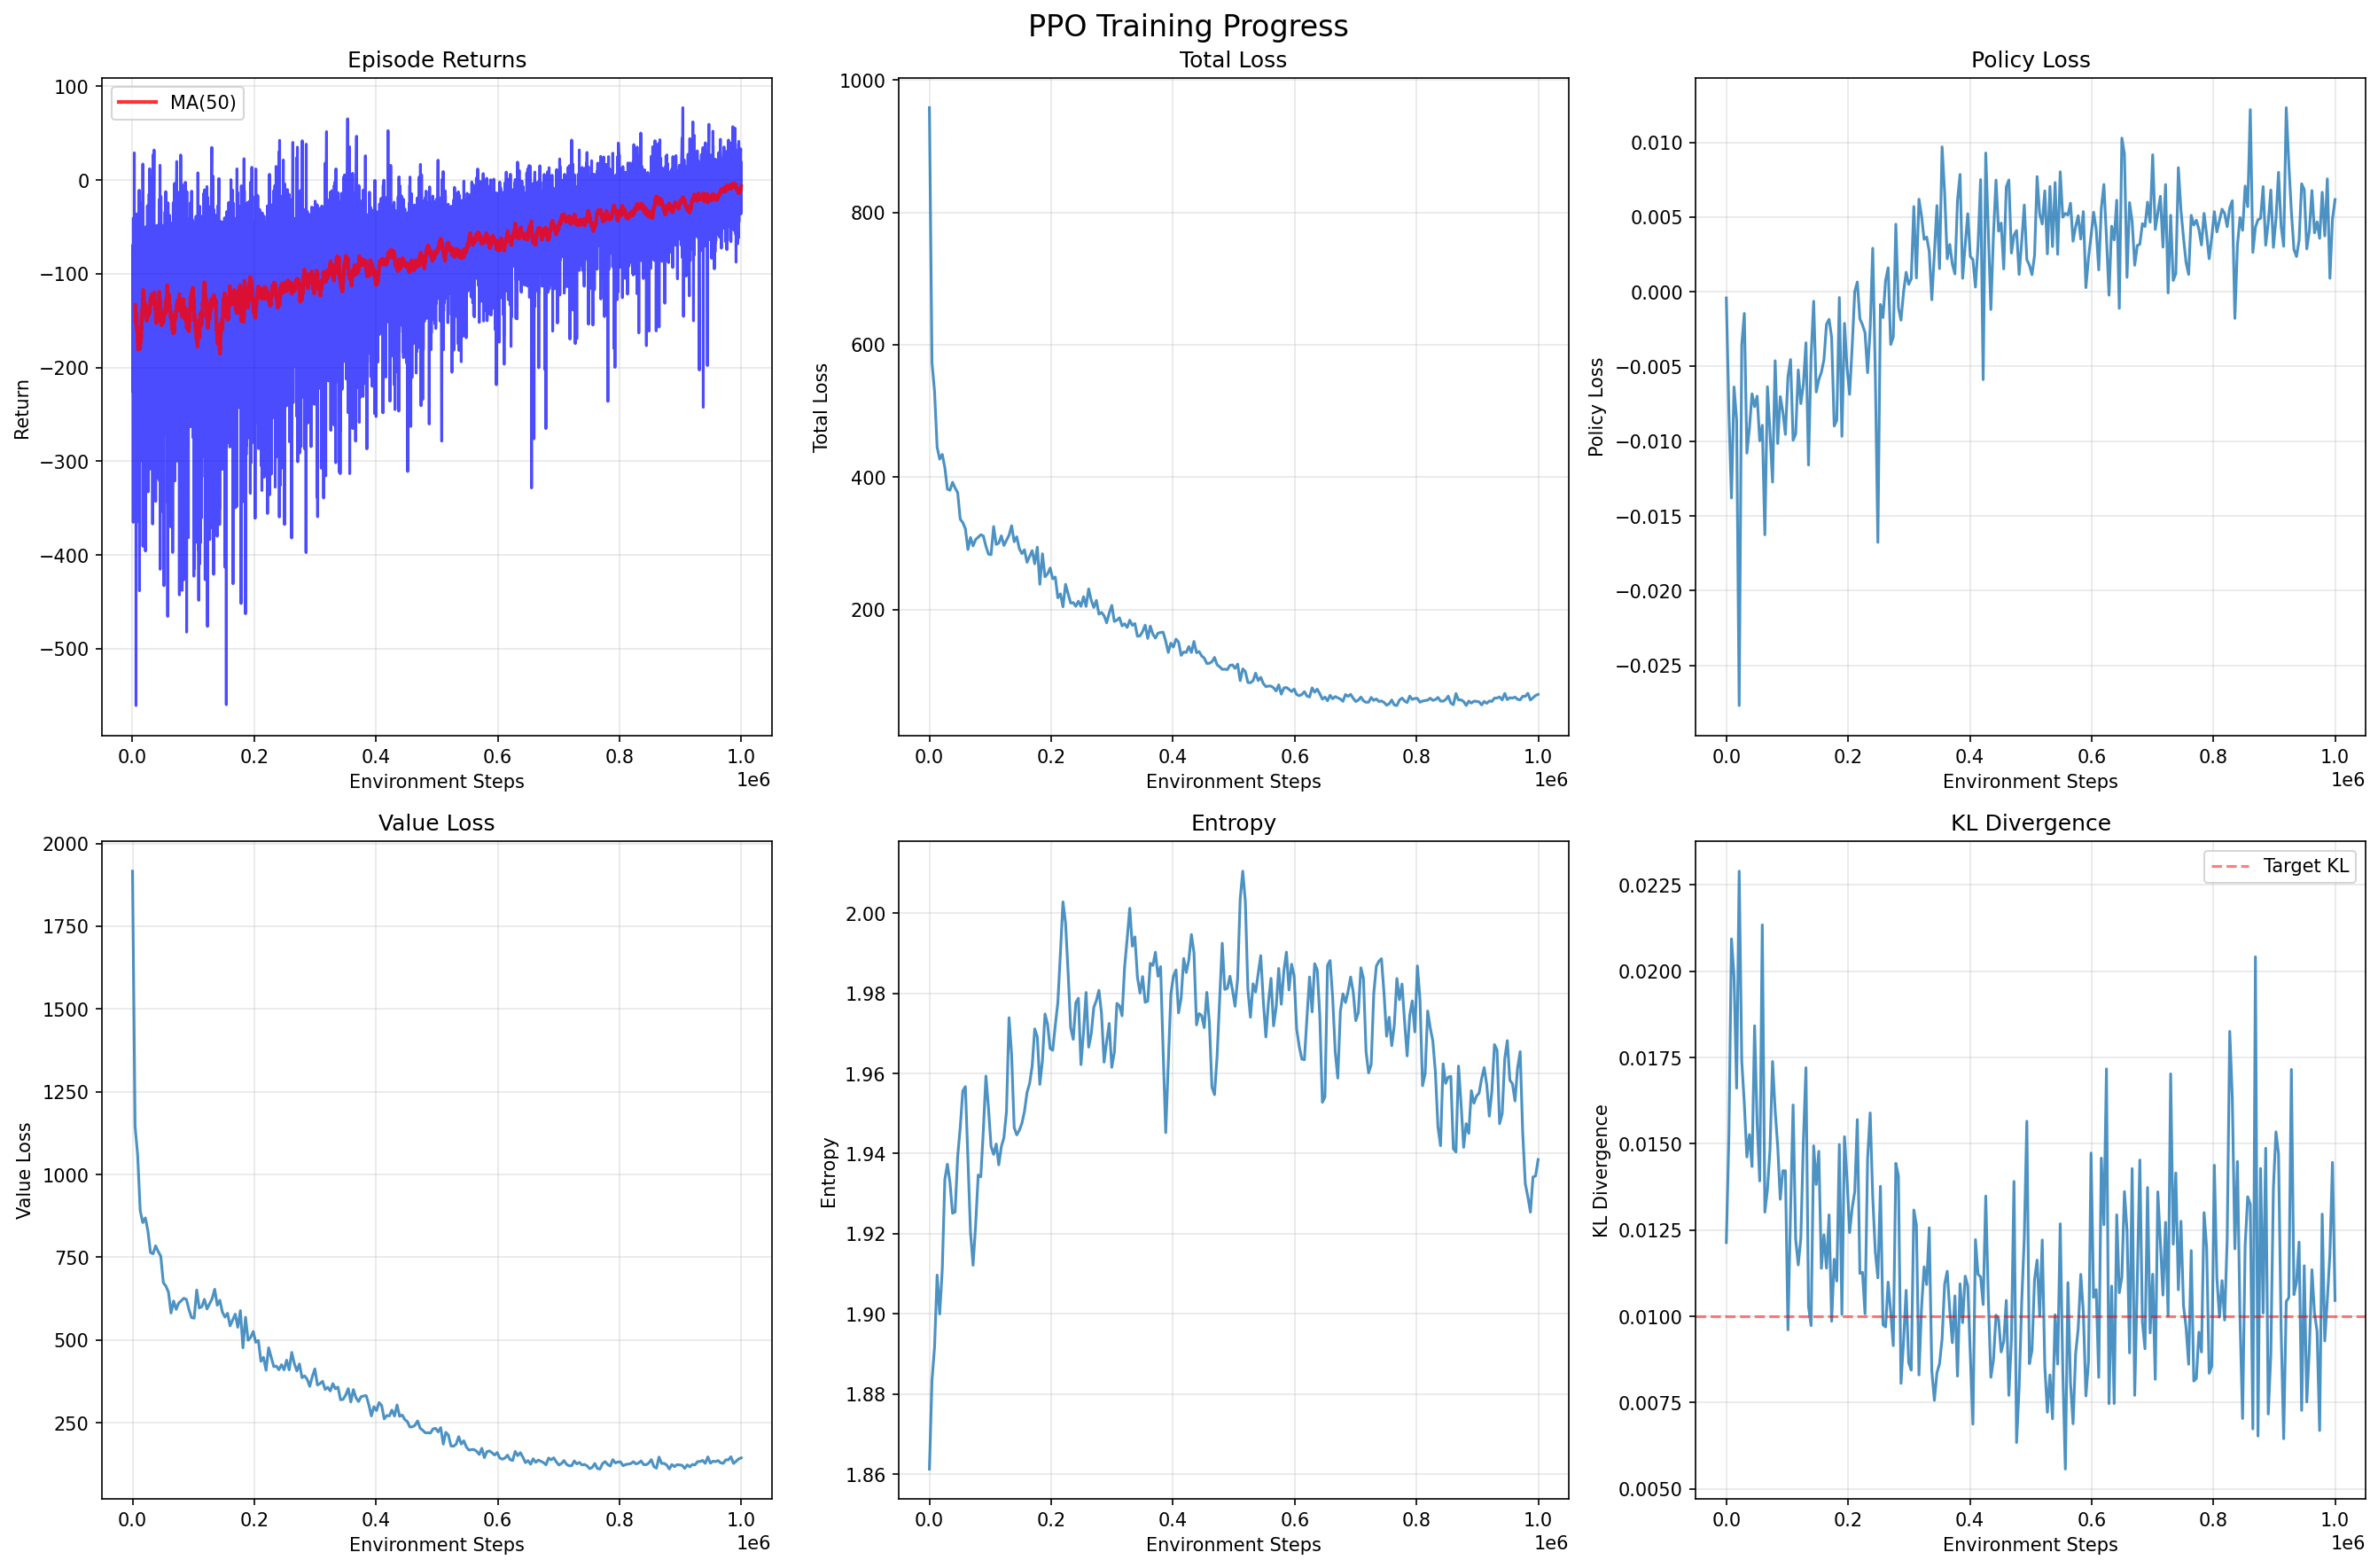
\includegraphics[width=\linewidth,height=8.5cm,keepaspectratio]{src/runs/ppo_images/1.6.1_training_curves.png}
\end{answerbox}
\boxlabel{Final return}
\begin{answerbox}{2cm}
\emph{Training:} Ending MA(50) = $-6.5$. Training returns (max/mean/min): all episodes $77.3/-82.5/-560.8$; last 50 $41.4/-6.5/-67.9$ (SD $25.1$).\par
\emph{Evaluation:} Best checkpoint, deterministic actions: $-113.3\pm 81.4$ (mean $\pm$ SD).\par
\end{answerbox}
\boxlabel{Discussion}
\begin{answerbox}{6.5cm}
\small{
Full replay performed worse than 1.4.1 with the ending MA(50) being $-6.5$ as compared to $142.3$, and the best checkpoint evaluation was $-113.3$ while 1.4.1 was $214.9$. Losses decreased relatively smoothly, and last-50 return SD was only $25.1$. However, KL remained around $0.01$ with repeated spikes (higher than $0.05$ in 1.4.1). Therefore, smooth losses and low return variability do not imply good / efficient learning here with same compute budget.

Older trajectories were collected by policies that chose different actions and visited different states. Their stored advantages and value targets may therefore be less relevant to the current policy. The probability ratio accounts for changes in action probabilities at each sampled state, but does not account for how often the current policy visits that state (\textbf{state visitation}). So, replay can direct updates toward states that matter less to the current policy.

Using \emph{more recent trajectories} and recomputing advantages and value targets with some off policy corrections could improve learning.
}
\end{answerbox}

\clearpage
\subproblem{1.6.2 Half Off-Policy PPO}{\ptsHalfOff}
\boxlabel{Plots}
\begin{answerbox}{9cm}
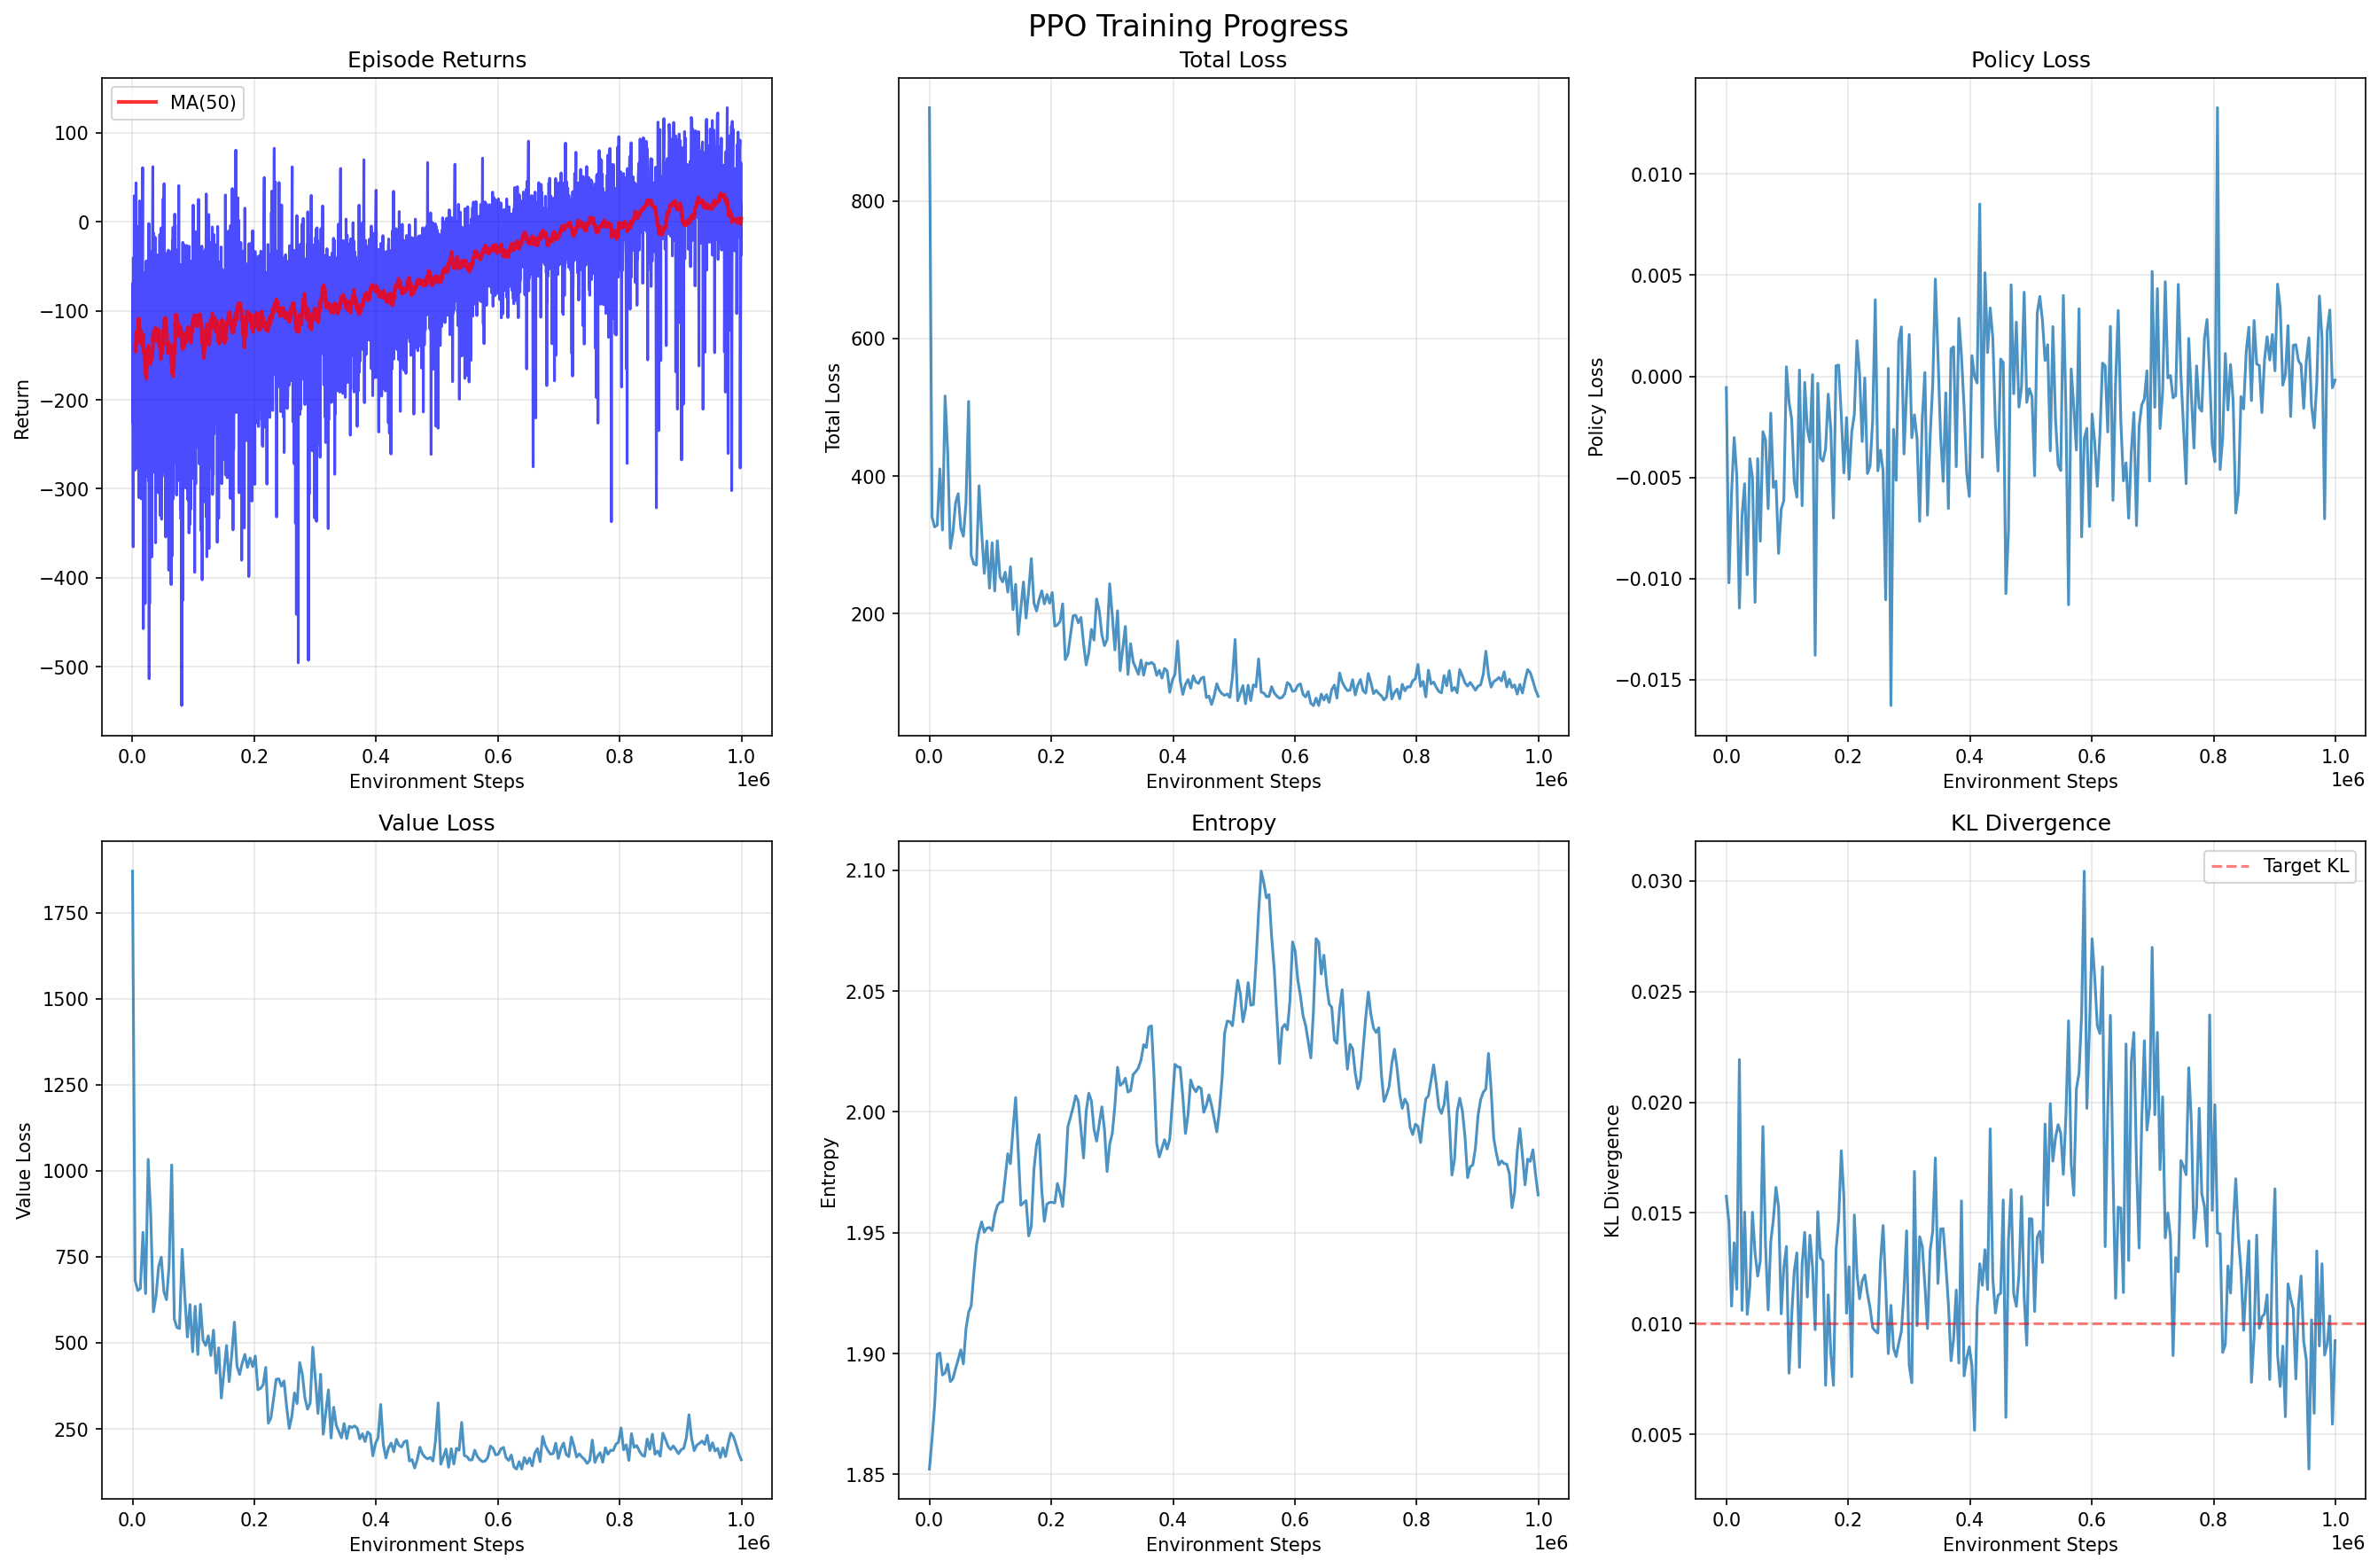
\includegraphics[width=\linewidth,height=8.5cm,keepaspectratio]{src/runs/ppo_images/1.6.2_training_curves.png}
\end{answerbox}
\boxlabel{Final return}
\begin{answerbox}{2cm}
\emph{Training:} Ending MA(50) = $3.3$. Training returns (max/mean/min): all episodes $128.1/-75.4/-543.4$; last 50 $128.1/3.3/-302.1$ (SD $92.9$).\par
\emph{Evaluation:} Best checkpoint, deterministic actions: $-100.2\pm 55.0$ (mean $\pm$ SD).\par
\end{answerbox}
\boxlabel{Discussion}
\begin{answerbox}{6.5cm}
Adding current-policy data modestly improved ending MA(50) from $-6.5$ to $3.3$, and best-checkpoint evaluation, from $-113.3$ to $-100.2$. However, it did not consistently improve stability since the graph shows larger late KL spikes. Last-50 return SD also increased from $25.1$ to $92.9$, with a minimum return of $-302.1$.

Fresh trajectories provide states and advantage estimates that better reflect the current policy, reducing some historical data mismatch and explaining the improved performance (referred to as state visitation in 1.6.1 answer). Replay still introduces some stale information and both variants remain far below the on-policy baseline (1.4.1). These results show that improved average performance need not come with smaller policy changes or more consistent episode returns.
\end{answerbox}

\clearpage
%% ===========================================================================
%% Problem 2: TD3
%% ===========================================================================
\problem{Problem 2: Twin Delayed DDPG -- TD3}{\ptsTDthree}

Problems 2.1--2.4 are graded from your code submission (\texttt{td3\_agent.py}) and have no
written component.

\subproblem{2.5 TD3 Evaluation}{\ptsTDEval}
\boxlabel{Plots}
\begin{answerbox}{10cm}
% YOUR SOLUTION HERE
\end{answerbox}
\boxlabel{Final performance}
\begin{answerbox}{2.5cm}
% YOUR SOLUTION HERE
\end{answerbox}

\clearpage
\subproblem{2.5 Target Policy Smoothing (\texttt{policy\_noise} $= 0$)}{\ptsTDSmooth}
\boxlabel{Plots}
\begin{answerbox}{9cm}
% YOUR SOLUTION HERE
\end{answerbox}
\boxlabel{Final performance}
\begin{answerbox}{2cm}
% YOUR SOLUTION HERE
\end{answerbox}
\boxlabel{Discussion}
\begin{answerbox}{6.5cm}
% YOUR SOLUTION HERE
\end{answerbox}

\clearpage
\subproblem{2.6 Policy Delay}{\ptsTDDelay}
\boxlabel{Plots: \texttt{--delay 1}}
\begin{answerbox}{9.5cm}
% YOUR SOLUTION HERE
\end{answerbox}
\boxlabel{Plots: \texttt{--delay 4}}
\begin{answerbox}{9.5cm}
% YOUR SOLUTION HERE
\end{answerbox}

\clearpage
\boxlabel{2.6 (continued) Final performance}
\begin{answerbox}{3.2cm}

\end{answerbox}
\boxlabel{Discussion}
\begin{answerbox}{8cm}
% YOUR SOLUTION HERE
\end{answerbox}

\clearpage
%% ===========================================================================
%% Problem 3: SAC
%% ===========================================================================
\problem{Problem 3: Soft Actor-Critic -- SAC}{\ptsSAC}

Problems 3.1--3.2 are graded from your code submission (\texttt{sac\_agent.py}) and have no
written component.

\subproblem{3.3 SAC Evaluation}{\ptsSACEval}
\boxlabel{Plots}
\begin{answerbox}{10cm}
% YOUR SOLUTION HERE
\end{answerbox}
\boxlabel{Final performance}
\begin{answerbox}{2.5cm}
% YOUR SOLUTION HERE
\end{answerbox}

\clearpage
\subproblem{3.4 UTD Ratio}{\ptsSACUTD}
\boxlabel{Plots: \texttt{--utd\_ratio 2}}
\begin{answerbox}{9.5cm}
% YOUR SOLUTION HERE
\end{answerbox}
\boxlabel{Plots: \texttt{--utd\_ratio 4}}
\begin{answerbox}{9.5cm}
% YOUR SOLUTION HERE
\end{answerbox}

\clearpage
\boxlabel{3.4 (continued) Final return and total run time}
\begin{answerbox}{3.2cm}
\end{answerbox}
\boxlabel{Analysis: sample efficiency vs.\ stability vs.\ wall-clock}
\begin{answerbox}{8cm}
% YOUR SOLUTION HERE
\end{answerbox}

\clearpage
\subproblem{3.5 Backup Action}{\ptsSACBackup}
\boxlabel{Plots}
\begin{answerbox}{10cm}
% YOUR SOLUTION HERE
\end{answerbox}
\boxlabel{Discussion (one to two sentences)}
\begin{answerbox}{4cm}
% YOUR SOLUTION HERE
\end{answerbox}

\clearpage
%% ===========================================================================
%% Problem 4: Feedback
%% ===========================================================================
\section*{Problem 4: Feedback}

\textbf{Feedback}: You can help the course staff improve the course by providing feedback.
What was the most confusing part of this homework, and what would have made it less
confusing?
\begin{answerbox}{4.5cm}
% YOUR SOLUTION HERE
\end{answerbox}

\textbf{Collaboration}: Detail the work division amongst your group below.
\begin{answerbox}{4.5cm}
% YOUR SOLUTION HERE
\end{answerbox}

\textbf{Time Spent}: How many hours did you spend working on this assignment? Your answer
will not affect your grade. Please average your answer over all the members of your team.
\begin{answerbox}{4.2cm}
\centering
\renewcommand{\arraystretch}{1.3}
\begin{tabular}{r|>{\centering\arraybackslash}m{2.5cm}}
Alone &
% YOUR SOLUTION HERE
\\ \hline
With teammates &
% YOUR SOLUTION HERE
\\ \hline
With other classmates &
% YOUR SOLUTION HERE
\\ \hline
At office hours &
% YOUR SOLUTION HERE
\\
\end{tabular}
\end{answerbox}

\end{document}